\subsection{Graphisches Ableiten}
Einen ungefähren Verlauf der Ableitungsfunktion kann man sich mit rein grafischen Überlegungen machen:
\begin{LA}{Einführungsbeispiel}{}
    In der folgenden Abbildung ist der Graph einer Funktion $f$ dargestellt. Skizzieren Sie den ungefähren Verlauf des Graphen der Ableitungsfunktion $f'$.
    \begin{center}
        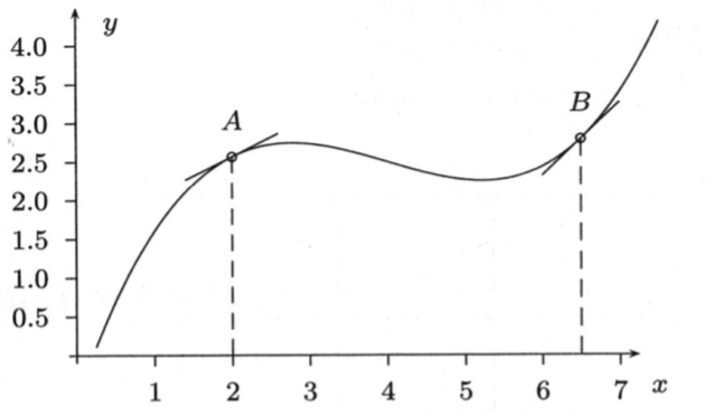
\includegraphics[scale = 1.3]{media/graphischesAbleiten.png}
    \end{center}
    \vspace{9
    cm}
\end{LA}
\begin{ueb}
    {}{}
    Siehe die Aufgaben im Buch Kapitel 3.2 (ab Seite 57).
\end{ueb} 